\chapter{Capacità descrittive del modello}\label{ch:descrizione}
In questo capitolo sono analizzate le capacità \textit{descrittive} del modello sviluppato. Gli errori di simulazione che si commettono quando i parametri del modello utilizzati per simulare una particolare seduta, sono ricavati dall'ottimizzazione della stessa specifica seduta, sono stati quantificati e analizzati nella loro distribuzione. Solo nel capitolo successivo saranno indagate le capacità \textit{predittive} del modello, ovvero saranno quantificati gli errori di simulazione che si commettono quando i parametri del modello sono ricavati dall'ottimizzazione sulle sedute precedenti dello stesso paziente.

\section{Calcolo degli errori}
Dopo aver ottimizzato i parametri di ogni seduta attraverso la procedura di ottimizzazione descritta nel Capitolo \ref{ch:ottimizzazione}, sono state effettuate le relative simulazioni ($6$ pazienti x $4$ sedute $=$ $24$ simulazioni, numero di prelievi per simulazione: variabile) e calcolati gli errori rispetto ai dati ematici. Se si indica con $y_{i,modello}$ la concentrazione plasmatica del soluto \textit{i} ricavata dalla simulazione, e con $y_{j,reale}$ la stessa concentrazione plasmatica ricavata dai dati ematici clinicamente rilevati, si può definire la seguente misura dell'errore percentuale di stima:
\begin{equation}\label{eq:errori}
	e_i = 100 \cdot \frac{y_{i,modello}-y_{i,reale}}{y_{i,reale}}
\end{equation}
Questo tipo di errore quantifica lo scarto simulazione-realtà e dà un informazione sulla direzione dello scarto: se positivo il dato simulato sovrastima il dato reale; viceversa se negativo il dato simulato sottostima il dato reale. In \tablename\ref{tab:descrizione} sono riassunti, per ogni soluto, i risultati relativi agli errori di stima $e_i$ in termini di media e deviazione standard della distribuzione di tali errori, più il valore massimo e minimo. Gli stessi indici sono stati calcolati per le distribuzioni formate dai valori assoluti degli errori di stima $|e_i|$. L'introduzione dei valori assoluti degli errori di stima si è resa necessaria per fornire un indice meno ambiguo che mostri le effettive capacità descrittive del modello: ipoteticamente, se ci fossero solo due valori da valutare e questi valori fossero pari a $+10\%$ e $-10\%$ la media di $e_i$ sarebbe zero, e si potrebbe erroneamente pensare che il modello in media non commetta errori. Questo non si verifica se si calcola la media degli elementi $|e_i|$. In altre parole, mentre il primo indice (cioè la media di $e_i$) fornisce una misura della \textit{polarizzazione} degli errori, il secondo (cioè la media di $|e_i|$) dà l'effettiva quantificazione degli errori di simulazione.
\begin{table}[htb]
	\centering
	\caption{Capacità descrittiva del modello: errori di stima $e_i$ ed errori assoluti di stima $|e_i|$. Media ($\mu$) e deviazione standard ($\sigma$). ($N_{sample}=87$).}\label{tab:descrizione}
	\begin{tabular}{lrrrrrrrr}
	\toprule 
		\textbf{Soluto}   &  \multicolumn{8}{c}{\textbf{Errori di simulazione (\%)}}  \\
		\cmidrule(lr){2-9}
				              &        \multicolumn{4}{c}{$e_i$}             &       \multicolumn{4}{c}{$|e_i|$}             \\
		                  & \multicolumn{1}{c}{$\mu$}      & \multicolumn{1}{c}{$\sigma$}   & $min$   & $max$   & \multicolumn{1}{c}{$\mu$}     & \multicolumn{1}{c}{$\sigma$}   & $min$   & $max$  \\
    \cmidrule(lr){2-5}\cmidrule(lr){6-9}
    %                    media       dev.std.        min        max    media ass   dev.st.        min       max
  	Sodio             & $ 0,11$     & $ 0,93$    & $ -1,93$  & $2,70$  & $0,78$   & $0,51$     & $0,01$ & $ 2,70$   \\
  	Potassio          & $-0,51$     & $ 4,44$    & $-11,86$  & $9,43$  & $3,33$   & $2,96$     & $0,02$ & $11,86$  \\
  	Cloro             & $-0,02$     & $ 0,59$    & $ -1,32$  & $1,82$  & $0,45$   & $0,37$     & $0,01$ & $ 1,82$   \\
  	Calcio            & $ 0,20$     & $ 1,91$    & $ -5,18$  & $10,62$ & $1,29$   & $1,42$     & $0,03$ & $10,62$  \\
  	Fosfato           & $ 1,92$     & $ 9,42$    & $-15,93$  & $32,98$ & $6,93$   & $6,62$     & $0,05$ & $32,98$  \\
  	Magnesio          & $ 3,10$     & $ 5,35$    & $ -7,94$  & $18,23$ & $4,80$   & $3,89$     & $0,05$ & $18,23$  \\
  	Urea              & $-3,13$     & $10,53$    & $-23,34$  & $18,83$ & $8,88$   & $6,40$     & $0,35$ & $23,34$  \\
  	Creatinina        & $-3,79$     & $10,03$    & $-26,67$  & $16,42$ & $8,83$   & $6,02$     & $0,06$ & $26,67$  \\
  	Proteine          & $ 7,10$     & $ 4,65$    & $ -3,32$  & $18,55$ & $7,23$   & $4,44$     & $0,16$ & $18,55$  \\
  \bottomrule
\end{tabular}
\end{table}

\begin{figure}[!h]
\centering
		\includegraphics[angle=-90, width=\textwidth]{immagini/err_sim.eps}
				\caption{Media + dev. st. degli errori di simulazione $|e_i|$ ($N_{sample}=87$).}\label{fig:err_pred}
\end{figure}

\section{Analisi dei risultati}
Prima di commentare i dati della \tablename~\ref{tab:descrizione} è doveroso fare una considerazione. Gli errori, calcolati secondo l'Eq.(\ref{eq:errori}), sono misure di scarto \textit{rapportate} al valore vero rispetto al quale si calcola lo scarto. Questo vuol dire che se il valore vero è molto alto, gli errori relativi tenderanno ad essere bassi, dando l'impressione che il modello simuli bene la realtà clinica. È questo il caso, ad esempio, del sodio per il quale il valore di riferimento è intorno alle $142$ $mmol/L$ (\tablename~\ref{tab:osmolarit}). Viceversa, quando il valore vero è molto basso lo scarto relativo diventa grande, dando l'impressione che il modello simuli male la realtà clinica. È questo il caso della creatinina per la quale il valore di riferimento è intorno alle $0,2$ $mmol/L$ (\textit{ibidem}). Con questa precisazione si vuole dare un ulteriore elemento che sia utile per l'interpretazione critica dei risultati.

\begin{description}
	\item[Proteine:] analizzando le medie degli errori di stima $e_i$, si nota che la concentrazione delle proteine è sempre sovrastimata. Si è individuato, a posteriori, che il \textit{bias} è dovuto alle ipotesi riguardanti la dinamica delle proteine: si era ipotizzato infatti che le proteine non fossero coinvolte in alcuno scambio di massa, perché ritenute non permeanti le membrane considerate nel modello (membrana capillare, cellulare, del dializzatore). La concentrazione plasmatica delle proteine quindi, poiché nel corso della dialisi il volume plasmatico diminuisce sempre, non può che aumentare. Questa ipotesi cade dopo che si controllano i risultati delle analisi del sangue effettuate sui campioni provenienti dalla realtà dialitica. In \figurename~\ref{fig:real_prot} sono mostrati i grafici relativi all'evoluzione della concentrazione plasmatica delle proteine di due sedute dialitiche di due diversi pazienti. 
\begin{figure}[!h]
	\centering
	\subfigure[]
	{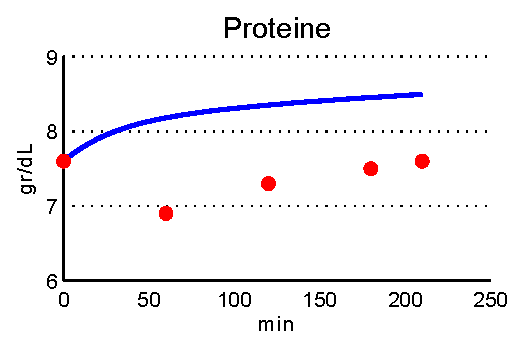
\includegraphics[width=0.4\textwidth]{immagini/protMAR4.eps}}\qquad
	\subfigure[]
	{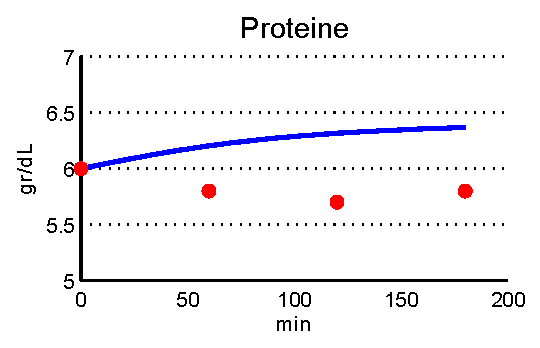
\includegraphics[width=0.4\textwidth]{immagini/protVAS2.eps}}
		\caption{Simulazione (linea continua) \textit{vs} dati clinici (puntini). La concentrazione plasmatica delle proteine nel corso della dialisi presenta valori inferiori rispetto a quelli iniziali, e ciò fa cadere le ipotesi fatte nel modello sulle proteine. (a) codice dialisi = MAR4, (b) codice dialisi = VAS2}\label{fig:real_prot}
\end{figure}
Si nota che tale concentrazione resta sempre al di sotto di quella a inizio seduta, fatto questo inspiegabile col modello attuale. Questo particolare andamento non emerge nei lavori precedenti riguardanti l'emodialisi \cite{casagrande, gatti}, nei quali le proteine tendono sempre a concentrarsi lungo il corso della seduta. È perciò possibile ipotizzare che questo comportamento sia tipico dell'HDF. Per quanto riguarda quindi la dinamica delle proteine è necessaria una modifica strutturale del modello. Delle modifiche che possono essere apportate sono (in ordine di plausibilità):
\begin{itemize}
	\item separare dalle proteine totali il contributo dell'albumina e considerare una possibile filtrazione di questa frazione proteica.
	\item introdurre un termine di perdita dal compartimento plasmatico che tenga conto dell'\textit{adsorbimento}\footnote{l'adsorbimento è il fenomeno attraverso il quale delle molecole restano adese ad una superficie. Per confermare l'esistenza di tale fenomeno potrebbe essere utile pesare il filtro dializzatore prima e dopo la dialisi.} delle proteine sulla membrana del dializzatore;
	\item verificare che il rapporto fra diluizione e ultrafiltrazione resti costante durante il corso della dialisi per escludere o includere un eventuale intervento della macchina dializzatrice nella determinazione degli scambi volumetrici;
	\item considerare che il sistema linfatico tende a creare uno spostamento di proteine fra plasma e interstizio bypassando la membrana capillare \cite{guyton}.
\end{itemize}
Nonostante le ipotesi riguardanti la dinamica delle proteine siano state invalidate dai dati clinici, considerando un valore di riferimento di circa $7$ $gr/dL$ l'errore massimo compiuto nella simulazione delle proteine, pari al $17\%$, corrisponde ad un errore sulla loro concentrazione di circa $1,26$ $gr/dL$, che secondo la formula di Landis-Pappenheimer, dà un contributo oncotico di circa $3$~$mmHg$, ben tamponato e compensato dai processi di feedback dell'organismo umano \cite{guyton}.
\begin{figure}[t]
	\centering
	\advance\leftskip-.2\textwidth
		\includegraphics[angle=-90, width=1.4\textwidth]{immagini/casi_peggiori.eps}
		\caption{Casi in cui l'errore di simulazione è massimo in valore assoluto (vedi l'ultima colonna di \tablename~\ref{tab:descrizione}). Simulazione (linea continua blu), dati veri (puntini rossi), punti di errore massimo (quadrati neri).}\label{fig:worst}
\end{figure}
\begin{figure}[t]
	\centering
	\advance\leftskip-.2\textwidth
		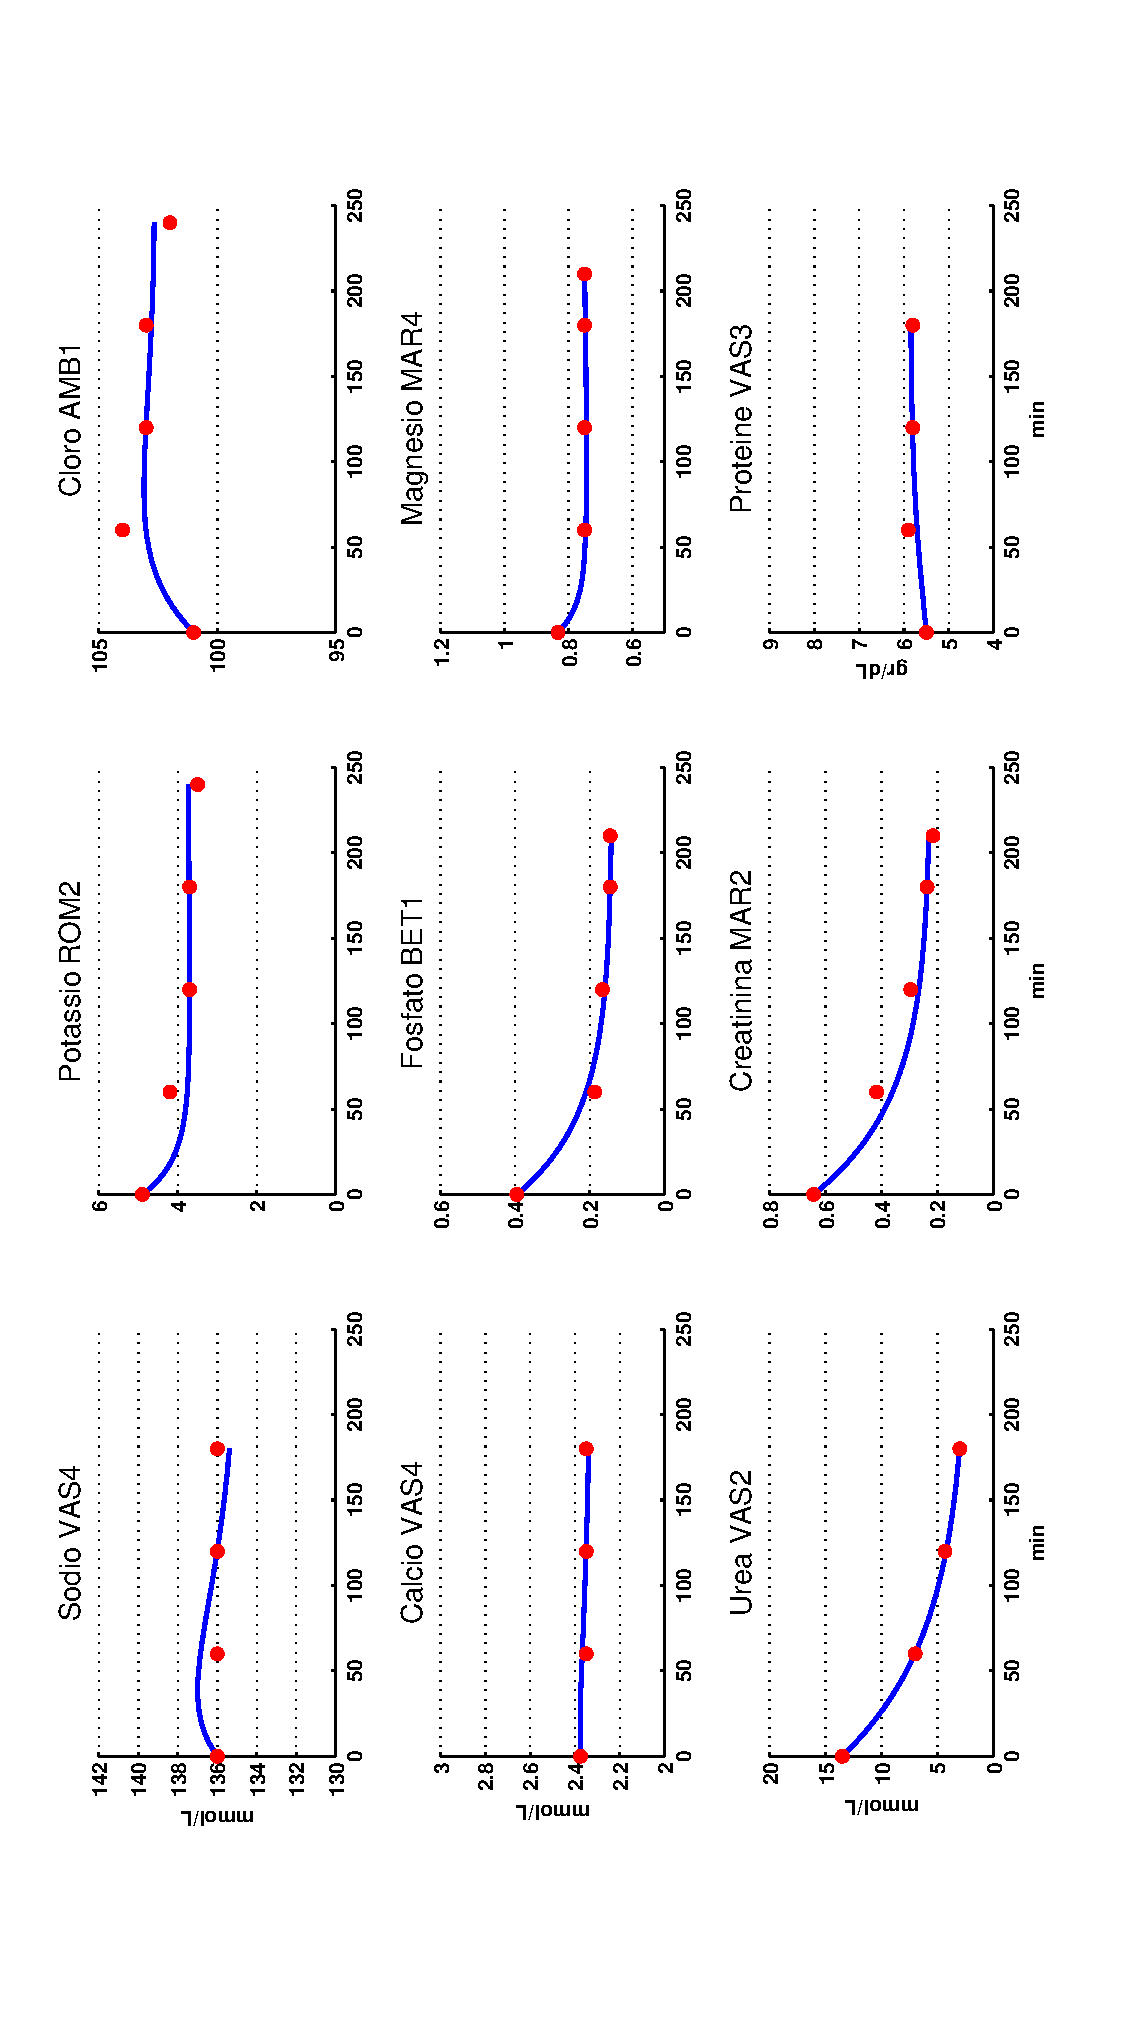
\includegraphics[angle=-90, width=1.4\textwidth]{immagini/casi_migliori.eps}
		\caption{Casi in cui l'errore di simulazione è minimo in valore assoluto. Simulazione (linea continua blu), dati veri (puntini rossi).}\label{fig:best}
\end{figure}
	\item[Sodio:] l'errore massimo in valore assoluto sul sodio è del $2,70\%$, il che potrebbe essere considerato accettabile. Se però si guarda alla \figurename~\ref{fig:worst}, si scopre che tale errore corrsponde a una sovrastima di $3,6$ $mmol/l$ della reale concentrazione plasmatica. Bisogna tener presente che uno dei sintomi più frequenti in dialisi sono i crampi muscolari, imputabili principalmente alle variazioni del sodio plasmatico e, sebbene l'HDF riduca tali sintomi rispetto all'emodialisi convenzionale \cite{evolutionHDF}, un errore nella predizione della dinamica del sodio potrebbe comportare, qualora un medico basasse le proprie decisioni sul modello descritto in questa tesi, l'insorgenza di crampi muscolari. Prima di decidere se un errore massimo del $2,70\%$ sul sodio è accettabile o meno, bisognerebbe stabilire quale sia la variazione accettabile sulla sua concentrazione plasmatica.
	\item[Potassio:] l'errore massimo in valore assoluto sul potassio è pari all'$11,86\%$ e corrisponde ad una sottostima di circa $0,49$ $mmol/L$ rispetto al valore vero. L'accettabilità dell'errore è subordinata all'accettabilità della sottostima. Il potassio è un soluto importante per la ritmicità del battito cardiaco e una decisione clinica basata su un errore di valutazione di questo soluto potrebbe a lungo termine constituire un pericolo per il paziente. Tuttavia, per le valutazioni di lungo termine dobbiamo considerare l'errore medio di simulazione sul soluto, che per il potassio vale $3,33\%$ (ca. $0,12$ $mmol/L$).
	\item[Cloro:] rammentando che, dopo quella del sodio, la concentrazione plasmatica basale del cloro è la più alta fra i restanti soluti, e che quindi bisogna porre attenzione alla valutazione degli errori, l'errore massimo in valore assoluto sul cloro è dell'$1,82\%$ (ca. $1,77$ $mmol/L$), e sembra quindi essere il soluto meglio simulato dal modello. 
	\item[Calcio:] unico fra gli elettroliti in virtù dell'enorme differenza di concentrazione fra l'esterno e l'interno della cellula\footnote{il calcio intracellulare è quasi inesistente. Nel modello il calcio intracellulare è stato inizializzato con il valore \texttt{eps}, che in Matlab rappresenta il limite di precisione numerica.}, il calcio ha un ruolo cruciale nell'accoppiamento eccitazione-contrazione nella muscolatura scheletrica, miocardica e liscia \cite{guyton}. Eventuali problematiche di ipo- o iper-calciemia si sviluppano nel lungo termine, il che ci permette di usare come valutazione della bontà del modello l'errore medio assoluto\footnote{dopo aver anche verificato che in nessun paziente ci siano delle deviazioni preferenziali, cioè sempre superiori o sempre inferiori, rispetto allo scostamento medio.}, pari per il calcio plasmatico all'$1,42\%$ (ca. $0,24$ $mmol/L$).
	\item[Magnesio:] nel caso presentato in \figurename~\ref{fig:worst} la dinamica simulata del magnesio è completamente diversa da quella reale: la prima è crescente mentre la seconda decrescente e l'errore assoluto massimo è pari al $18,23\%$. Fra tutte le $24$ sedute analizzate, solo in altri quattro casi si nota un andamento analogo. Nelle restanti $19$ sedute si ha un andamento simile a quello di \figurename~\ref{fig:best}. Valutazioni cliniche erronee basate sulla simulazione di questo soluto potrebbero non avere conseguenze gravi in quanto la quantità di magnesio plasmatico corrisponde a solo il $3,7\%$ circa del magnesio totale nell'organismo (\tablename~\ref{tab:osmolarit}) e che il magnesio legato nell'osso rappresenta un \textit{pool} rapidamente scambiabile che funge da riserva per mantenere costante la concentrazione extracellulare di magnesio \cite{guyton}. Quest'ultima considerazione suggerisce che un modo per migliorare la simulazione di questo soluto è quello di usare un modello a tre compartimenti che tenga conto dell'interazione del magnesio col sistema osseo. Un'alternativa possibile è quella di rimuovere questo soluto dal modello sviluppato. Il contributo del magnesio sull'osmolarità plasmatica totale ammonta ad appena lo $0,27\%$ (\tablename~\ref{tab:osmolarit}) e pertanto un'esclusione di questo soluto dal modello non comporterebbe variazioni significative sugli altri soluti.
	\item[Fosfato:] è il soluto in cui gli errori assoluti sono fra i più dispersi e di cui l'errore massimo supera il $30\%$. È anche il soluto che, insieme alla creatinina, ha la concentrazione plasmatica basale più bassa, e ciò contribuisce sicuramente ad amplificare la misura, effettuata secondo l'Eq.~\ref{eq:errori}, degli errori di simulazione. La causa può anche essere attribuita alla modellizazione della cinetica del soluto. Infatti, nella letteratura medica \cite{bib:fosfato} il fosfato plasmatico, durante il corso della dialisi, presenta un andamento bifasico decrescente/crescente, tale per cui se la concentrazione del fosfato scende al di sotto di una certa soglia, entra in azione un meccanismo che tende a farne rialzare la concentrazione plasmatica. Effettivamente possiamo constatare che in alcuni pazienti (esempio in \figurename~\ref{fig:real_fos}), la concentrazione a fine dialisi del fosfato è superiore rispetto alle rilevazioni immediatamente precedenti. Per ridurre gli errori nella simulazione del fosfato, bisognerebbe considerare di implementare un modello a tre o addirittura quattro compartimenti, come è stato fatto in lavori precedenti riguardanti l'emodialisi \cite{SilvTer, merulla}. Dalla \tablename~\ref{tab:distrib} si può tuttavia constatare che a fine dialisi nessun errore sul fosfato supera il $20\%$ e che oltre la metà di essi è comunque inferiore al $5\%$.
\begin{figure}[!h]
	\centering
	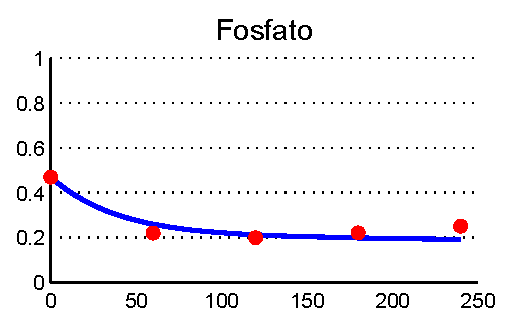
\includegraphics[width=0.4\textwidth]{immagini/fosAMB3.eps}
	\caption{Simulazione (linea continua) \textit{vs} dati clinici (puntini). Il fosfato reale mostra un andamento bifasico modellizzabile con l'introduzione di altri compartimenti. Codice dialisi: AMB3.}\label{fig:real_fos}
\end{figure}
	\item[Urea:] l'errore massimo in valore assoluto sull'urea è del $23,34\%$ ($1,4$ $mmol/L$ ). Il punto in cui è calcolato questo errore corrisponde alla seconda ora della seduta dialitica (\figurename~\ref{fig:worst}). Per questo soluto è più importante valutare la concentrazione a fine dialisi in quanto è il valore col quale il paziente lascia la seduta dialitica e che tenderà ad aumentare fino alla seduta successiva. Come si vede dalla \tablename~\ref{tab:distrib} a fine dialisi oltre il $50\%$ degli errori commessi è inferiore al $10\%$ che corrisponde a circa $0,4$ $mmol/L$ (rif. a fine dialisi di $4$ $mmol/L$).
\begin{table}[!t]
	\centering
	\caption{Distriduzione degli errori di simulazione dopo un ora e alla fine della seduta dialitica.}\label{tab:distrib}
	\begin{tabular}{lrrrrrrrr}
	\toprule 
		\textbf{Soluto}   &  \multicolumn{8}{c}{\textbf{Distribuzione degli errori di simulazione $|e_i|$ (\%)}}  \\
		\cmidrule(lr){2-9}
				              &        \multicolumn{4}{c}{$60$ $min$}          &       \multicolumn{4}{c}{fine dialisi}             \\
		                  & \multicolumn{1}{c}{\scriptsize$\leq 5\%$}      & \multicolumn{1}{c}{\scriptsize$5-10\%$}   & \multicolumn{1}{c}{\scriptsize$10-20\%$}  & \multicolumn{1}{c}{\scriptsize$>20\%$}     & \multicolumn{1}{c}{\scriptsize$\leq 5\%$}      & \multicolumn{1}{c}{\scriptsize$5-10\%$}   & \multicolumn{1}{c}{\scriptsize$10-20\%$}   & \multicolumn{1}{c}{\scriptsize$>20\%$}  \\
    \cmidrule(lr){2-5}\cmidrule(lr){6-9}
    Sodio          & $100,00$ & $-$     & $-$     & $-$     & $100,00$ & $-$     & $-$     & $-$ \\
  	Potassio       & $54,17$  & $25,00$ & $20,83$ & $-$     & $66,67$  & $33,33$ & $-$     & $-$ \\
  	Cloro          & $100,00$ & $-$     & $-$     & $-$     & $100,00$ & $-$     & $-$     & $-$ \\
  	Calcio         & $95,83$  & $-$     & $4,17$  & $-$     & $95,83$  & $4,17$  & $-$     & $-$ \\
  	Fosfato        & $33,33$  & $8,33$  & $45,83$ & $12,50$ & $54,17$  & $29,17$ & $16,67$ & $-$ \\
  	Magnesio       & $45,83$  & $50,00$ & $4,17$  & $-$     & $50,00$  & $29,17$ & $20,83$ & $-$ \\
  	Urea           & $29,17$  & $33,33$ & $33,33$ & $4,17$  & $37,50$  & $20,83$ & $41,67$ & $-$ \\
  	Creatinina     & $20,83$  & $41,67$ & $33,33$ & $4,17$  & $20,83$  & $41,67$ & $37,50$ & $-$ \\
  	Proteine       & $20,83$  & $45,83$ & $33,33$ & $-$     & $45,83$  & $37,50$ & $16,67$ & $-$ \\
\bottomrule
\end{tabular}
\end{table}
	\item[Creatinina:] l'errore massimo in valore assoluto sulla creatinina è del $26,67\%$ ($0,06$ $mmol/L$ ). Il punto in cui è calcolato questo errore corrisponde alla prima ora della seduta dialitica (\figurename~\ref{fig:worst}). Per questo soluto, come per l'urea, è più importante valutare la concentrazione a fine dialisi in quanto è il valore col quale il paziente lascia la seduta dialitica e che tenderà ad aumentere fino alla seduta successiva. Come si vede dalla \tablename~\ref{tab:distrib} anche per la creatinina a fine dialisi oltre il $50\%$ degli errori commessi è inferiore al $10\%$, che corrisponde a circa $0,02$ $mmol/L$ (rif. a fine dialisi di $0,2$ $mmol/L$).
\end{description}

La valutazione della bontà del modello non può basarsi, per quanto anticipato all'inizio del paragrafo,  solo sull'analisi degli errori percentuali, perché si corre il rischio di dare poco peso agli errori più gravi in termini di $mmol/L$ (e.g. sodio), oppure di criticare scostamenti che gravi potrebbero non essere (e.g. fosfato, urea, creatinina). Per questo si è cercato, in queste pegine, di fornire anche considerazioni di tipo clinico, che siano di ausilio, dove possibile, per la corretta interpretazione degli errori di simulazione.
